In questo capitolo parleremo in maniera più approfondita del linguaggio Vadalog e di tutte le sue particolarità. \newline
Vadalog è un linguaggio che raggiunge un attento equilibrio tra espressività e complessità, e può essere utilizzato come reasoning core di un KGMS. Fa parte della famiglia Warded Datalog$^\pm$ un frammento della famiglia Datalog$^\pm$. \newline 
Il capitolo è organizzato come segue. Nella sezione 1.1 verrà descritto in maniera approfondita il core del linguaggio, sono presenti tre sezioni, una che descrive il core logico dei linguaggi appartenenti alla famiglia di linguaggi Datalog$^\pm$, una che descrive il core logico di Vadalog, e come soddisfa la decidibilità, infine è presente una sezione per descrivere la complessità del core logico Vadalog.
Nella sezione 1.2 è possibile trovare dei programmi Vadalog di esempio per una maggiore comprensione del linguaggio. \newline
Questo capitolo prende spunto da diversi articoli pubblicati dal gruppo VADA, sia per alcune nozioni teoriche che per esempi pratici descritti~\cite{bellomarini2017swift, gottlob2015beyond}.

\section{Il core del linguaggio}

Il linguaggio Vadalog, fa parte della famiglia di linguaggi Warded Datalog$^\pm$, che a sua volta rappresenta un frammento della famiglia di linguaggi Datalog$^\pm$, ovvero una restrizione della famiglia Datalog$^\pm$, in particolare garantendone la decidibilità. \newline
In questa sezione andremo a focalizzarci proprio su tali famiglie di linguaggi e le relative complessità, la sezione 1.1.1 che descrive il core logico dei linguaggi Datalog$^\pm$, tutte le proprietà e i vincoli che esso induce, la sezione 1.1.2 che descrive il core logico di Vadalog, le proprietà della famiglia Warded Datalog$^\pm$, la sezione 1.1.3 che descrive la complessità e le caratteristiche del linguaggio Vadalog, infine la sezione 1.1.4, dove vengono descritte le estensioni adottate dal linguaggio Vadalog che introducono funzionalità aggiuntive al linguaggio base.\newline

\subsection{Il core logico dei linguaggi Datalog$^\pm$}

L'obiettivo principale dei linguaggi Datalog$\pm$ è quello di estendere il noto linguaggio Datalog con funzionalità di modellazione utili come quantificatori esistenziali nelle teste delle regole (il + nel simbolo $\pm $), e contemporaneamente limitare la sintassi della regola, in modo tale che sia garantita la decidibilità e la tracciabilità dei dati del reasoning (il - nel simbolo $\pm $). \newline
Il core dei linguaggi Datalog$\pm $ è costituito da regole note come \emph{regole esistenziali}, che generalizzano le regole Datalog con quantificatori esistenziali nelle teste delle regole, un esempio di regola esistenziale: \[Person(x) \rightarrow \exists y ~HasFather(x,y), Person(y)\]
che esprime che ogni persona, ha un padre e che anche questo a sua volta è una persona. \newline
In generale, una regola esistenziale è una formula del primo ordine: \[\forall \bar{x} \forall \bar{y} (\phi(\bar{x}, \bar{y}) \rightarrow \exists \bar{z} \psi (\bar{x}, \bar{z})\]
dove $\phi$ il corpo) e $\psi$  (la testa) sono congiunzioni di atomi con costanti e variabili. \newline
La semantica dell'applicazione di un insieme di regole esistenziali $\Sigma$ su un database $D$, in simboli $\Sigma$(D), è definita mediante una procedura di \emph{chase}~\cite{fagin2005data}. Durante questa procedura vengono aggiunti nuovi atomi a D (coinvolgendo anche valori nulli per soddisfare le variabili esistenziali), finché il risultato finale $\Sigma$(D) non soddisfa tutte le regole esistenziali. \newline
Vediamo un esempio di tale procedura: \newline
Consideriamo un Database D = \{Person(Bob)\}, e la regola esistenziale: \[Person(x) \rightarrow \exists y ~HasFather(x,y), Person(y)\]
L'atomo del database D innesca la regola esistenziale e vengono aggiunti i seguenti atomi: \[HasFather(Bob, \nu_{1}) ~e~ Person(\nu_{1})\]
$\nu_{1}$ è un \emph{labeled null} che rappresenta un valore sconosciuto.\newline
Il nuovo atomo Person($\nu_{1}$) innesca nuovamente la regola esistenziale, e vengono aggiunti altri atomi a D: \[HasFather(\nu_{1}, \nu_{2}) ~e~ Person(\nu_{2})\]
Dove $\nu_{2}$ è un nuovo nullo. Il risultato è l'istanza: \[\{Person(Bob), HasFather(Bob, \nu_{1})\} \cup \underset{i>0}{\bigcup} ~\{Person(\nu_{i}), HasFather(\nu_{i}, \nu_{i+1})\}\]
$\nu_{1}$, $\nu_{2}$, ..., $\nu_{i}$, $\nu_{i+1}$ sono labeled nulls. \newline \newline
Data una coppia Q=($\Sigma$, Ans), dove $\Sigma$ è un insieme di variabili esistenziali e Ans un predicato n-ario, la valutazione di Q su un database D, indicata Q(D), è definita come set di tuple sopra sopra l'insieme $C_{d}$ di valori costanti che occorrono nel database D. \newline
Il compito principale del reasoning è \emph{l'inferenza di tuple}: dato un database D, una coppia Q = ($\Sigma$, Ans), ed una tupla di costanti $\bar{t}$, bisogna decidere se $\bar{t}$ appartiene a Q. Questo problema è molto difficile, infatti è indecidibile, anche quando Q è fissato e solo D è dato come input~\cite{cali2013taming}. \newline
Ciò ha portato all'attività di identificare restrizioni sulle regole esistenziali che rendono tale problema decidibile. Ciascuna di queste restrizioni genera un nuovo linguaggio della famiglia Datalog$\pm$. \newline

\subsection{Il core logico di Vadalog}

Vadalog è un linguaggio logico e rappresenta un'estensione di Datalog, quindi un programma Vadalog è composto da un insieme di regole. \newline
In ogni regola è possibile trovare una testa ed un corpo, nel quale ogni testa è composta da un insieme di atomi ed ogni corpo da un insieme di atomi e un insieme di condizioni. Gli atomi del corpo possono essere: atomi di input (che traggono i loro fatti direttamente dalla persistenza), atomi già presenti in teste di altre regole o nella regola stessa (ricorsione). \newline 
Ogni atomo può essere composto da un numero indefinito di argomenti, che possono essere variabili o costanti. \newline
Riportiamo un esempio di regola contenente atomi composti da variabili e costanti: \[a(X) :- b(X,``Hi")\]
Poiché Vadalog appartiene alla famiglia di linguaggi Warded Datalog$^\pm$, contiene quantificatori esistenziali nelle teste, che generano valori nulli. \newline
Nel linguaggio Vadalog, ci sono tre tipologie di variabili:

\begin{enumerate}
	\item \emph{Harmless}: Variabili standard presenti nel corpo di una regola, che non possono assumere valori nulli.
	\item \emph{Harmful}: Rappresentano dei nulli presenti nel corpo di una regola, e che sono a loro volta prodotti da un quantificatore esistenziale nella testa di un'altra regola.
	\item \emph{Dangerous}: Sono le variabili i cui valori, potenzialmente nulli, si propagano nella testa delle regola.
\end{enumerate}

Vadalog si basa sulla nozione di \emph{wardedness}, proprietà ereditata dalla famiglia di linguaggi Warded Datalog$^\pm$~\cite{gottlob2015beyond}. \newline
La wardedness applica una restrizione su come vengono utilizzate le variabili "\textit{dangerous}" (pericolose) di un insieme di regole esistenziali. Intuitivamente una variabile dangerous è una variabile del corpo che può essere unificata con un valore nullo quando viene applicato l'algoritmo di ricerca e viene propagato anche alla testa della regola.\newline
Per esempio dato l'insieme $\Sigma$ di regole esistenziali \[P(x) \rightarrow \exists z~R(x,z)~e~R(x,y) \rightarrow P(y)\]
La variabile y nel corpo della seconda regola è dangerous. Dato un database D = \{P(a)\}, il chase applica la prima regola e genera R(a, $\nu$), dove $\nu$ è un nullo che funge da testimone della variabile esistenziale \textit{z}, e poi la seconda regola verrà applicata con la variabile \textit{y} che è unificata con $\nu$ che viene propagata all'atomo ottenuto P($\nu$). \newline

\begin{figure}[h!]
	\centering
	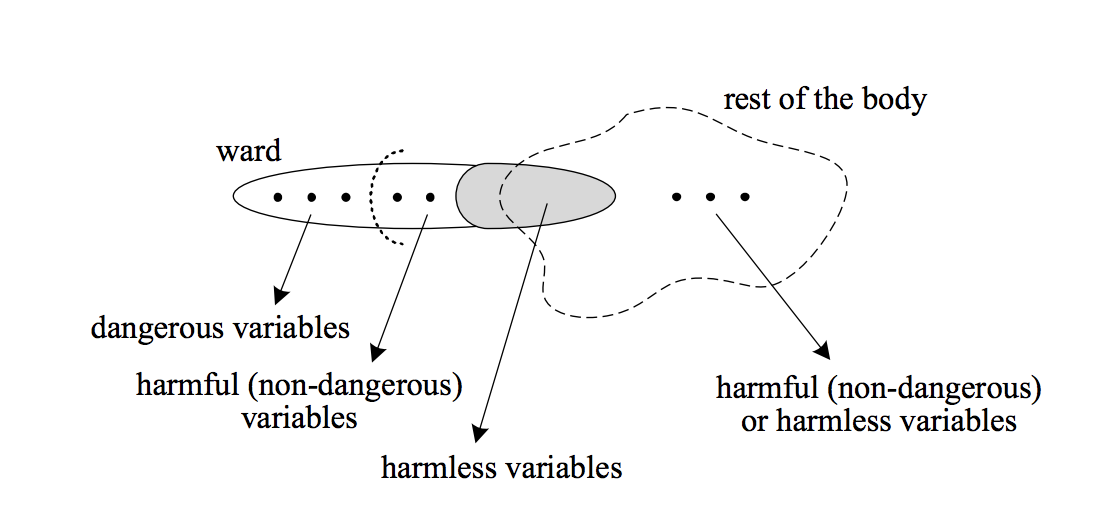
\includegraphics[width=0.8\linewidth]{figure/wardedness}
	\caption{Corpo di una regola warded~\cite{gottlob2015beyond}.}
	\label{fig:wardedness}
\end{figure}
L'obiettivo della wardedness è quello di porre dei vincoli sulla modalità in cui i valori nulli vengono propagati come segue: 
\begin{enumerate}
	\item  Tutte le variabili dangerous devono coesistere in un singolo corpo di un atomo A, chiamato il ward;
	\item Il ward può condividere solo variabili \textit{harmless} con il resto del corpo.
\end{enumerate}
Una regola è warded se vengono rispettate entrambe le condizioni appena citate. In Figura~\ref{fig:wardedness} possiamo vederne una rappresentazione grafica. \newline

\subsection{Complessità}

In questa sezione viene descritta la complessità di Warded Datalog$^\pm$, anche facendo riferimenti a possibili frammenti di esso. \newline
Warded Datalog$^\pm$ è composto da insiemi (finiti) di regole esistenziali warded, esso rappresenta un raffinamento di \textit{Weakly-Frontier-Guarded Datalog$\pm$}, che è una famiglia di linguaggi definita allo stesso modo ma senza la condizione 2 citata nella sezione 1.1.2~\cite{baget2011rules}.
Weakly-Frontier-Guarded Datalog$\pm$ è intrattabile nella complessità dei dati, infatti è EXPTIME-completo. \newline \newline
Warded Datalog$\pm$ gode di diverse proprietà che lo rendono robusto ed utilizzabile in pratica:
\begin{itemize}
	\item L'inferenza di tuple è trattabile; infatti essa è PTIME-completa quando l'insieme di regole è fisso.
	\item Cattura Datalog, senza incrementare la complessità. Infatti un insieme $\Sigma$ di regole Datalog è implicitamente Warded poiché non ci sono variabili dangerous per definizione.
	\item Generalizza linguaggi ontologici principali come OWL 2 QL (linguaggio ontologico per la semantica del web~\cite{OWL2QL})
	\item È adatto per la ricerca di grafi RDF (Resource Description Framework, strumento base proposto da W3C per la codifica, scambio e riutilizzo di metadati~\cite{RDFW3C}). In realtà aggiungendo la negazione stratificata, si ottiene un linguaggio chiamato TriQ-Lite1.0~\cite{gottlob2015beyond}, che può esprimere ogni query SPARQL (linguaggio di query per gli RDF~\cite{SPARQLW3C}) nell'ambito del regime di OWL 2 QL.
\end{itemize}

Anche se la data complexity di Vadalog è accettabile per applicazioni convenzionali, può risultare inadatta per applicazioni Big Data. \newline
Ciò solleva il problema relativo all'esistenza di frammenti di Warded Datalog$^\pm$ che garantiscano una minore complessità dei dati, ma mantengano allo stesso tempo le proprietà descritte in precedenza. \newline
Tale frammento di Warded Datalog$^\pm$, definito "\emph{StronglyWarded}", dovrebbe avere complessità NLOGSPACE e si potrebbe ottenere limitando il modo in cui viene utilizzata la ricorsione. Prima di dare la definizione di StronglyWarded diamo la nozione di grafo dei predicati. \newline
Il grafo dei predicati di $\Sigma$, chiamato PG($\Sigma$), è un grafo diretto (V,E), in cui l'insieme dei nodi V è composto da tutti i predicati presenti in $\Sigma$, ed abbiamo un arco da un predicato P ad un predicato R se esiste $\sigma \in \Sigma$ tale che P è presente nel corpo di $\sigma$ ed R è presente nella testa di $\sigma$. Si consideri un insieme di nodi S $\subseteq$ V e un nodo R $\in$ V, diciamo che R è $\Sigma$-raggiungibile da S se esiste almeno un nodo P $\in$ S che può raggiungere R attraverso un percorso in PG($\Sigma$). \newline
Possiamo ora introdurre la definizione di \emph{strong wardedness}. Un insieme di regole esistenziali $\Sigma$ viene chiamato strongly-warded se $\Sigma$ è warded e per ogni $\sigma \in \Sigma$ nella forma \[\phi(\bar{x}, \bar{y}) \rightarrow \exists \bar{z} P_{1}(\bar{x}, \bar{y}), ..., P_{n}(\bar{x}, \bar{y})\] esiste al massimo un atomo di $\phi(\bar{x}, \bar{y})$ il cui predicato è $\Sigma$-raggiungibile da \{$P_{1}, ..., P_{n}$\}. \newline
Strongly-Warded Datalog$^\pm$ è composto da insiemi finiti di regole esistenziali che sono strongly-warded. \newline
Intuitivamente, in un insieme di regole esistenziali strongly-warded, ogni regola $\sigma$ non è ricorsiva. Si può quindi dimostrare che il nostro principale compito, l'inferenza di tuple nel processo di reasoning, in Strongly-Warded Datalog$^\pm$ è NLOGSPACE nella complessità dei dati. Inoltre questo linguaggio raffinato rimane abbastanza potente per catturare OWL 2 QL e esteso con una lieve negazione può esprimere ogni query SPARQL. \newline
Come detto in precedenza, la complessità dei dati NLOGSPACE esclude immediatamente il datalog completo. Tuttavia Strongly-Warded Datalog$^\pm$ include alcuni importanti e ben studiati frammenti di Datalog:
\begin{itemize}
	\item \emph{Datalog non ricorsivo}, dove il grafo dei predicati è quindi aciclico.
	\item \emph{Linear Datalog}, in cui ogni regola può avere al massimo un predicato nel suo corpo.
\end{itemize}
Per ottenere il core logico di Vadalog, i linguaggi appena discussi, ovvero Warded, Strongly-Warded e Linear Datalog$^\pm$, sono arricchiti di utili funzionalità senza pagarne un prezzo in complessità. \newline
Infatti si considerano i vincoli negativi della forma $\forall \bar{x}(\phi(\bar{x}) \rightarrow \bot)$, dove $\phi$ è una congiunzione di atomi e $\bot$ denota la costante false. Vengono presi in considerazione anche i vincoli di uguaglianza (come condizioni) della forma $\forall \bar{x}(\phi(\bar{x}) \rightarrow x_{i} = x_{j})$, dove $\phi$ è una congiunzione di atomi e $x_{i}$ e $x_{j}$ sono variabili di $\bar{x}$, che non interagiscono con le regole esistenziali. Questa classe di vincoli di uguaglianza è conosciuta come non conflittuale~\cite{cali2012towards}, ovvero senza conflitti con variabili esistenziali. \newline
Si noti che se consideriamo vincoli arbitrari di uguaglianza, senza restrizioni, allora il nostro compito di reasoning diventa indecidibile~\cite{chandra1985implication}.

\subsection{Estensioni di Vadalog}

Al fine di essere efficace per applicazioni nel mondo reale, il core logico di Vadalog descritto in precedenza è stato esteso con un insieme di funzionalità aggiuntive di utilità pratica, che risultano essenziali per permettere un'analisi più dettagliata sui dati. Nel seguito della sezione elenchiamo tutte le estensioni che sono state applicate in Vadalog. \newline \newline
\emph{Tipi di dato}: È possibile definire costanti e variabili. Il linguaggio supporta i tipi di dato più comuni: Integer, Float, String, Boolean, Date, ma esiste anche il supporto per tipi di dato compositi, come i Set. \newline \newline
\emph{Espressioni}: Le variabili e le costanti possono essere combinate in espressioni, definite ricorsivamente come variabili, costanti o combinazioni di esse, per le quali supportiamo molteplici operazioni per diversi tipi di dato: somma, moltiplicazione, divisione, per Integer e Float; contenimento, aggiunta, cancellazione degli elementi per i Set; operazioni su stringhe (contains, starts-with, ends-with, index-of, substring, ecc.), operazioni sui booleani (and, or, not, ecc.). \newline
Le espressioni possono essere usate nei corpi di regola come lato sinistro (LHS) di una condizione, cioè il confronto (<,>,=,<=,>=,<>) di una variabile del corpo con l'espressione stessa o come LHS di un'assegnazione, cioè la definizione di un valore calcolato specificatamente, spesso utilizzata come variabile di testa quantificata esistenzialmente. \newline \newline
\emph{Funzioni di Skolem}: I valori dei nulli possono essere calcolati con funzioni. Si presume che siano deterministici (restituendo un nullo univoco) e avere range disgiunti. Alle funzioni di Skolem è possibile applicare delle implementazioni procedurali, che possono essere definite in diversi linguaggi, definendo il calcolo che effettuerà la funzione. \newline \newline
\emph{Aggregazioni monotone}: Vadalog supporta l'aggregazione (min, max, somma, prodotto, conteggio), mediante un'estensione alla nozione di aggregazioni monotone~\cite{shkapsky2015optimizing}, che consente di adottare l'aggregazione anche in presenza di ricorsioni. Le recenti applicazioni di Vadalog in casi di utilizzi industriali impegnativi hanno dimostrato che tali aggregazioni sono molto efficienti in vari scenari Big Data del mondo reale. \newline \newline
\emph{Annotazioni}: Gli atomi nelle regole sono decorati con annotazioni, in modo che un passo nel processo di reasoning innesca il componente esterno. Le fonti di dati e gli obiettivi possono essere dichiarati adottando annotazioni di input/output. Le annotazioni sono fatti particolari che aumentano le serie di regole esistenti con comportamenti specifici. Ad esempio una semplice annotazione che può essere di input/output, può prendere/persistere i dati da un sistema esterno, come un database relazionale. I fatti possono essere quindi derivati, per esempio da un database relazione o un graph db, che vengono acceduti con le due annotazioni di esempio, rispettivamente:
\begin{lstlisting}
	@bind("Own", "rdbms", "companies.ownerships")
\end{lstlisting}
\begin{center}
\begin{tabular}{c}
\begin{lstlisting}
@qbind("Own", "graphDB", 
"MATCH (a) - [o:Owns] -> (b) 
RETURN a, b, o.weight"). 
\end{lstlisting}
\end{tabular}
\end{center}
Dove la prima annotazione effettua una proiezione di tutta la tabella "ownerships", mentre nella seconda viene effettuata una vera e propria query a Neo4J, uno specifico database a grafo, in Cypher (linguaggio per interrogazione di Neo4J). \newline
Un approccio simile viene utilizzato anche per supportare le piattaforme di machine learning esterne e di estrazione dati nel sistema. Facciamo un esempio, utilizzando il framework di estrazione dati OXPath~\cite{furche2013oxpath}, un'estensione di XPath (linguaggio che permette di individuare nodi all'interno di un documento XML) che interagisce con le applicazioni web per estrarre le informazioni ottenute durante la navigazione web. \newline
Supponiamo che le nostre informazioni sulla proprietà di un'azienda siano parziali, mentre le altre informazioni possono essere reperite dal web. In particolare, supponiamo che un registro aziendale agisca come motore di ricerca web, prendendo come input un nome di un'azienda e restituendo come pagine separate le società di proprietà. Queste informazioni possono essere ottenute come segue:
\begin{lstlisting}
	@qbind("Own", "oxpath", 
	"doc('http://company_register.com/ownerships') 
	/descendant::field()[1]/{$1} 
	/following::a[.#='Search']/{click/} 
	/(//a[.#='Next']/{click/})* 
	//div[@class='c']:<comp> 
	[./span[1]:<name=string(.)>] 
	[./span[3]:<percent=string(.)>]"). 
\end{lstlisting}
Interazioni interessanti si possono osservare in scenari più sofisticati, in cui il processo di reasoning e l'elaborazione dei componenti esterni sono più intrecciati. \newline
Inoltre è possibile definire delle annotazioni di mapping, che hanno lo scopo di definire diverse informazioni sui dati di output, ad esempio i tipi, il nome delle colonne di destinazione, la posizione, ecc., ma possono essere anche evitati, poiché il sistema è in grado di inferire il tipo di dato. \newline \newline
\emph{Reasoning probabilistico}: Vadalog offre il supporto per i casi di base in cui è possibile garantire il calcolo scalabile. I fatti sono considerati probabilisticamente indipendenti ed una forma minimalistica di inferenza probabilistica è offerta come risposta alla query. I fatti possono essere adornati con misure di probabilità. \newline
Quindi se l'insieme delle regole esistenziali rispetta specifiche proprietà sintattiche che garantisco il calcolo probabilistico, i fatti risultanti della query sono arricchiti dalla loro probabilità marginale. \newline
Nell'esempio utilizziamo il probabilistic reasoning per tenere conto delle proprietà incerte (ad esempio a causa di fonti inaffidabili), stabilendo i fatti con la loro probabilità, per trarre conclusioni sui rapporti di controllo aziendali:
\begin{lstlisting}
	0.8 :: Own("ACME", "COIN", 0.7) 
	0.3 :: Own("COIN", "SAVERS", 0.3) 
	0.4 :: Own("ACME", "GYM", 0.55) 
	0.6 :: Own("GYM", "SAVERS", 0.4)
\end{lstlisting}
\emph{Post-processing Annotations}: Spesso è necessario dopo il processo di reasoning effettuare delle semplici operazioni utili per l'utente finale. \newline
In Vadalog queste operazioni sono delle annotazioni, che rientrano nella categoria delle Post-processing annotations. La particolarità di queste annotazioni è che non aumentano la complessità computazionale del sistema, poiché effettuate dopo il processo di reasoning. Degli esempi di post-processing annotations sono orderby, rimozione dei duplicati, e tanti altri. \newline \newline
Nel complesso, il linguaggio supporta il reasoning basato sulla logica e il machine learning in tre modi. In primo luogo, il linguaggio supporta l'inferenza probabilistica in casi di base come visto in precedenza. \newline
In secondo luogo, le estensioni del linguaggio di base forniscono tutte le funzionalità necessarie per estrarre e incorporare algoritmi avanzati di inferenza in modo che possano essere eseguiti direttamente dal sistema Vadalog e quindi sfruttare le proprie strategie di ottimizzazione. \newline
Infine, per le applicazioni di machine learning più sofisticate, le estensioni consentono una semplice interazione con librerie e sistemi specializzati.

\section{Esempi di programmi Vadalog e loro utilizzo}

In questa sezione verranno presentati diversi programmi Vadalog di esempio, utilizzati per effettuare calcoli particolari ed utilizzare alcune delle estensioni descritte sopra, e spiegati nel dettaglio. \newline
Partiremo da esempi molto semplici, dove interagiscono pochi elementi (join tra due elementi), fino ad arrivare ad esempi più complessi che utilizzano ricorsione, espressioni, funzioni di skolem, integrazione di database, post processing annotations e così via. \newline
Un primo esempio di un programma Vadalog molto semplice:
\begin{example}\label{esempio_1}
\begin{lstlisting}

	a(1,0). 
	b(1,2). 
	c(X,Y,Z) :- a(X,Y), b(X,Z). 
	@output("c").
\end{lstlisting}
\end{example}
Nell'esempio~\ref{esempio_1} viene effettuato il join tra gli atomi a e b, sulla prima variabile e vengono proiettate tutte le variabili. In questo caso, i fatti di input vengono aggiunti manualmente a(1,0) e b(1,2), quindi il risultato sarà c(1,0,2). \newline
I join possono coinvolgere anche più atomi tra di loro, e possono essere abbinati anche alla ricorsione, nel seguente esempio ne vediamo un'applicazione:
\begin{example}\label{esempio_2}
\begin{lstlisting}

a(1.0,"string"). 
b(1.0,2). 
c(1.0,4,2017-09-28 12:29:00). 
c(X,Y,W) :- a(X,Y), b(X,Z), c(X,V,W). 
@post("unique", "c"). 
@output("c").
\end{lstlisting}
\end{example} 
Nell'esempio~\ref{esempio_2}, viene effettuato il join tra tre atomi, di cui uno ricorsivo, vengono dati i fatti di input (anche un input per 'c'), e viene eseguita anche un'operazione di post-processing 'unique' che ha l'obiettivo di rimuovere i duplicati. \newline
I fatti di input in questo caso sono vari: double, interi, stringhe e date. Come detto in precedenza, oltre ad essere dichiarati esplicitamente come fatti possono rappresentare tabelle su un database, relazionale e non, o anche le righe di un file csv, ecc. \newline
Attraverso questa integrazione è possibile effettuare delle statistiche incrociando dati provenienti da storage distinti, combinando dati, e producendo dati di output che possono rappresentare nuova conoscenza, alla base del processo di reasoning. \newline
Infatti è anche possibile direzionare gli output verso una determinata fonte, oltre la stampa a schermo. È possibile salvare un output ad esempio in un database, in un file csv e quant'altro. \newline 
Questo risulta molto importante poiché uno degli obiettivi del processo di reasoning è produrre nuova conoscenza, analizzando ed incrociando dati già acquisiti. \newline 
 Nell'esempio~\ref{esempio_3} vedremo un'interazione che può avvenire tra diverse sorgenti dati all'interno di un programma Vadalog con persistenza del risultato: 
\begin{example}\label{esempio_3}
\begin{lstlisting}

@input("a"). 
//a composto da due colonne 
@bind("a", "postgres", "vadaschema", "Table"). 
@input("b"). 
//b composto da due colonne 
@bind("b", "csv", "absolute/path/to/folder", "filename.csv"). 
c(X,Y,Z) :- a(X,Y), b(X,Z). 
@output("c"). 
@bind("c", "csv", "absolute/path/to/folder", "result.csv").
\end{lstlisting}
\end{example} 
Dove i fatti di input vengono presi da un database postgres (con schema "vadaschema" e tabella "Table") contenente due colonne e da un file csv (che è nella directory "absolute/path/to/folder" chiamato "filename.csv") contenente anch'esso due elementi per riga. Viene poi effettuato il join tra i due input in base al primo elemento, ed il risultato viene salvato in un nuovo file csv, che viene appositamente creato nella directory "absolute/path/to/folder". \newline 
C'è anche la possibilità di effettuare delle preselezioni dal database, con un'annotazione chiamata \emph{qbind}, che permette di effettuare una vera e propria query in SQL, ne vediamo un utilizzo nell'esempio~\ref{esempio_4}:
\begin{example}\label{esempio_4}
\begin{lstlisting}

@input("a"). 
//a composto da due colonne 
@qbind("a", "postgres", "vadaschema", 
"select name1, name2
from Table
where name1 = 'teststring'"). 
@input("b"). 
//b composto da due colonne 
@bind("b", "csv", "absolute/path/to/folder", "filename.csv"). 
c(X,Y,Z) :- a(X,Y), b(X,Z). 
@output("c"). 
@bind("c", "csv", "absolute/path/to/folder", "result.csv").
\end{lstlisting}
\end{example} 
È anche possibile inserire delle espressioni all'interno dei programmi Vadalog, esse possono essere utilizzate, come condizioni o assegnazioni di una variabile esistenziale. Per entrare più nel dettaglio vediamo qualche esempio: 
\begin{example}\label{esempio_5}
\begin{lstlisting}

a(1,5). 
b(2,7). 
c(X,V) :- a(X,Y), b(V,W), Y >= 5, W >= 5. 
@output("c"). 
\end{lstlisting}
\end{example} 
Nell'esempio~\ref{esempio_5} sono presenti due condizioni Y >= 5 e W >= 5, quindi la proiezione in 'c' viene fatta soltanto se entrambe sono verificate, poiché Y e W, con i fatti specificati valgono 5 e 7, le condizioni sono verificate e quindi l'output sarà c(1,2). \newline
\begin{example}\label{esempio_6}
\begin{lstlisting}

a(1,5). 
b(2,7). 
c(X,V,J) :- a(X,Y), b(V,W), J = X+V. 
@output("c").
\end{lstlisting}
\end{example}
Nell'esempio~\ref{esempio_6} invece le espressioni vengono utilizzate per assegnare un valore ad una variabile esistenziale, in questo caso J=X+V, quindi l'output sarà c(1,2,3). \newline
È possibile integrare skolem function (che vengono considerate come espressioni), al quale è possibile applicare delle funzioni esterne con cui possono essere definite, o altrimenti generano un nullo. Vediamo qualche applicazione negli esempi~\ref{esempio_7} e \ref{esempio_8}:
\begin{example}\label{esempio_7}
\begin{lstlisting}

b(1,2). 
a(X,Y,Z) :- b(X,Y),Z=\#f(X,Y). 
c(K) :- b(X,Y),K=\#f(X,Y). 
d(K) :- b(X,Y),K=\#g(X,Y). 
@output("a"). 
@output("c"). 
@output("d"). 
\end{lstlisting}
\end{example}
\begin{example}\label{esempio_8}
\begin{lstlisting}

b(1,2). 
c(3,2). 
a(Y,Z) :- b(X1,Z),c(X2,Z),Y=\#f(X1,X2). 
@output("a"). 
@implement("\#f","java","com.package1.package2.myClass","staticmethodName").
\end{lstlisting}
\end{example}
Nell'esempio~\ref{esempio_7} non vengono definite le implementazioni delle funzioni, quindi ritorneranno un valore nullo, \#f(X,Y) rappresenta una funzione in questo esempio. La particolarità delle funzioni è che se in due regole la stessa funzione prende come input gli stessi valori, allora quest'ultima produrrà lo stesso nullo. In questo esempio il risultato prodotto sarà a(1,2,$z_{1}$), c($z_{1}$) e d($z_{2}$), dove $z_{1}$ e $z_{2}$ rappresentano i nulli. 
Nell'esempio~\ref{esempio_8} invece, la funzione 'f' viene implementata attraverso una procedura esterna (in questo caso un metodo Java) del quale non entriamo nel dettaglio implementativo, ma il risultato della funzione Java sarà lo stesso risultato di 'f'.